\section{The Research Map method}
\label{sec:method}

\subsection{Origin, sources, and purpose}

The Research Map is a method for structuring a proposed academic research project. Its primary source is a teaching map prepared by Sergio Fran\c{c}a in August 2026; a subsequent methodological specification makes the intended dependencies and review points more explicit \cite{franca2026map,franca2026detail}. The method is motivated by a practical planning difficulty: a broad theme, a central problem, objectives, chapter topics, and methods can be drafted separately without a clear account of how one leads to another. A later author-supplied application export articulates this concern in terms of students' difficulty beginning and organizing a project. We treat that account as a design motivation, not as a measured frequency of difficulties, delays, or educational outcomes.

The two primary documents have different roles. The initial map is a compact template that numbers five stages and places the objective--method matrix beside the specific objectives. The later specification describes rules of dependency, an origin--destination traceability map, coherence questions, and points at which a researcher may validate or revise proposed content. Some passages of the later document describe capabilities a supporting system \emph{should} have. In this section they are reported as part of the methodological specification, not as evidence that the application implements every capability. Section~\ref{sec:system} will examine that correspondence separately.

\subsection{Five stages and their relations}

The map begins with one central research problem: a question that gives the project its focus. The detailed specification suggests producing alternatives from the researcher's context, theme, or keywords, then selecting a definitive formulation for subsequent steps \cite{franca2026detail}. It recommends beginning that question with expressions equivalent to ``How'' or ``In what way''. This is a local drafting convention intended to elicit a researchable relation, not a universal requirement for scientific questions. The researcher's selection and revision of the problem remain substantive decisions.

A single general objective should respond to the selected problem and state the intended overall result of the project. The specification recommends an infinitive verb and uses the general objective as a basis for a provisional title \cite{franca2026map,franca2026detail}. The general objective is then decomposed into three to six specific objectives. Each should contribute a step toward the overall aim, rather than introduce an unrelated project. The detailed specification illustrates four specific objectives, but four is a suggested starting configuration within the original range, not a new fixed count.

The fourth stage organizes literature-review topics from the problem, keywords, and objectives. The initial map suggests three to six such topics. The fifth stage organizes development or analysis topics from the objectives, including the general objective where appropriate \cite{franca2026map}. A specific objective may be addressed principally through the literature review or through later development or analysis, depending on its role. The suggestion that a final development topic reconnect to the general objective is guidance for a coherent exposition, not a rule that every disciplinary article must follow. The map's stages describe relationships among planning elements; they need not be read as an irreversible sequence of writing operations.

\begin{table}[htbp]
\centering
\small
\caption{The five numbered stages in the original Research Map and their planning relations. The objective--method matrix is a companion element, not a sixth stage.}
\label{tab:method-stages}
\begin{tabular}{p{0.25\linewidth} p{0.34\linewidth} p{0.31\linewidth}}
\hline
Stage & Planning artifact & Principal relation \\
\hline
1. Research problem & One selected central question & Establishes the project's focus \\
2. General objective & One overall intended aim & Responds to the problem; informs the provisional title \\
3. Specific objectives & Three to six contributing steps & Decompose the general objective \\
4. Literature topics & Thematic review outline & Draws on the problem, keywords, and relevant objectives \\
5. Development / analysis topics & Outline for later analysis or development & Organizes the objectives to be addressed beyond the review \\
\hline
\end{tabular}
\end{table}

The detailed specification also treats research questions as an item for validation and revision \cite{franca2026detail}. They belong to the method's account of a research design, but they are not a sixth numbered stage in the initial map. This distinction matters when comparing the source method with the application, which presently has a central problem question but no separate research-questions unit.

\subsection{The objective--method matrix}

Beside the specific objectives, the original map places three planning questions: how information or data will be collected for each objective; how they will be analyzed or treated; and what result or impact is expected \cite{franca2026map}. This matrix connects a stated aim to a proposed means of addressing it. It can expose a missing collection procedure, an analysis that does not answer the objective, or an expected result that has no evident route from the planned work. These are issues for examination, not defects proven by the presence or absence of a filled cell.

The matrix is associated with the five stages rather than numbered as an additional stage. Its entries are prospective: \emph{expected result} names an anticipated output of a proposed study, not a finding already observed. In particular, completing this matrix does not establish that a method is feasible, that evidence will be obtained, or that an expected impact will occur. The researcher must judge the appropriateness of each collection and analysis choice in the project's disciplinary context.

\subsection{Dependencies, traceability, and human judgment}

The later specification represents the map as a set of origin--destination relations: inputs inform the selected problem; the problem informs the general objective; that objective informs the specific objectives; and the objectives guide literature and development topics \cite{franca2026detail}. It also proposes checking whether an objective has a corresponding topic, a plausible method, a collection procedure, an analysis, and an expected result. A traceability relation identifies why an item is present and what it is intended to address. It does not, by itself, establish conceptual coherence or scientific adequacy.

The specification therefore pairs suggested checks with researcher validation. The researcher may choose a problem from alternatives, adjust the general and specific objectives, revise research questions and topic structures, and assess the proposed methodological connections. The logic of dependency, traceability, coherence inspection, and human revision belongs to the method. A growing knowledge base, a comprehensive methodological library, and a rule engine are proposed means of supporting that logic; they are not additional numbered stages and should not be assumed to exist fully in the current software \cite{franca2026detail}.

\begin{figure}[htbp]
\centering
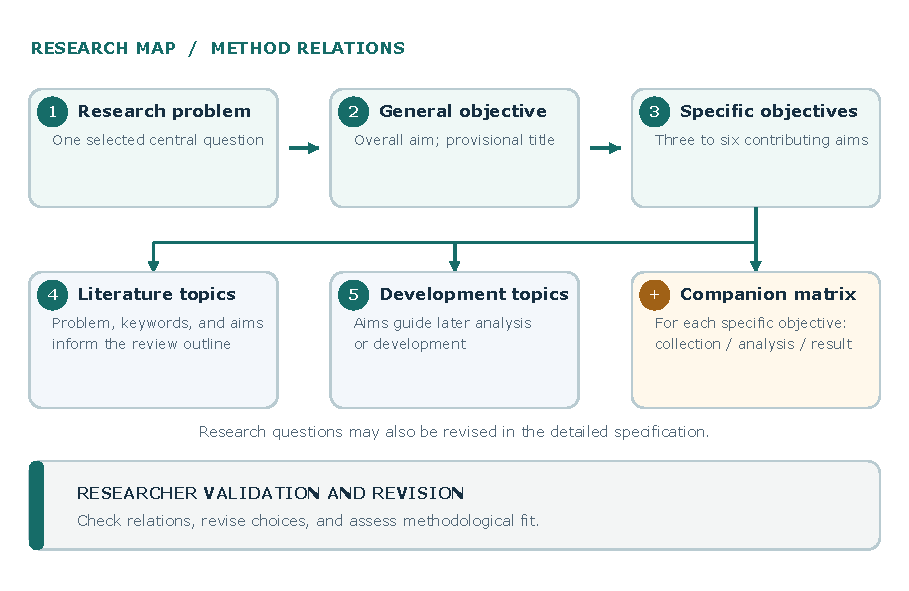
\includegraphics[width=\linewidth]{figures/method-flow.pdf}
\caption{Interpretive redrawing of the Research Map's five stages, companion matrix, and human revision. Arrows express methodological relations described in the primary documents; they do not represent observed application behavior or an irreversible workflow.}
\label{fig:method-flow}
\end{figure}

The method supplies a structured way to make planning decisions and their intended relations explicit. It does not offer a formal proof that a completed map yields a valid research design, nor does it evaluate the efficiency of planning. The next section examines which of these methodological relations are represented in the present application and agent, and where that representation is partial.
